\section{~\videojam{} Architecture}\label{sec:architecture}

This section presents the general design of~\videojam{}, a self-balancing architecture for live video analytics.~\videojam{} is designed around three design guidelines:
\begin{enumerate}[leftmargin=*]
    \item \textbf{Per-function type-based load balancing.} To cope with the heterogeneous performance profiles and highly variable workloads, we design~\videojam{} to implement a decentralized set of load balancers on a per-function type basis.
    \item \textbf{Short-term load forecasting.} To enhance frames offloading across functions but avoid errors from unreliable long-term trends, we design~\videojam{} to solely rely on short-term forecasting of incoming workload trends.
    \item \textbf{Robustness to configuration changes.} Finally, to work independently from variations in configurations changes and camera arrivals
    and departures, we design~\videojam{} to solely rely on observed performance patterns (\eg, incoming rate) rather than any pre-compute knowledge of
    deployment configuration.
\end{enumerate}

In the rest of the section, we first present the global overview of the~\videojam{} architecture, then describe in details the components of the system.

\subsection{System Overview}

\begin{figure}
    \centering
    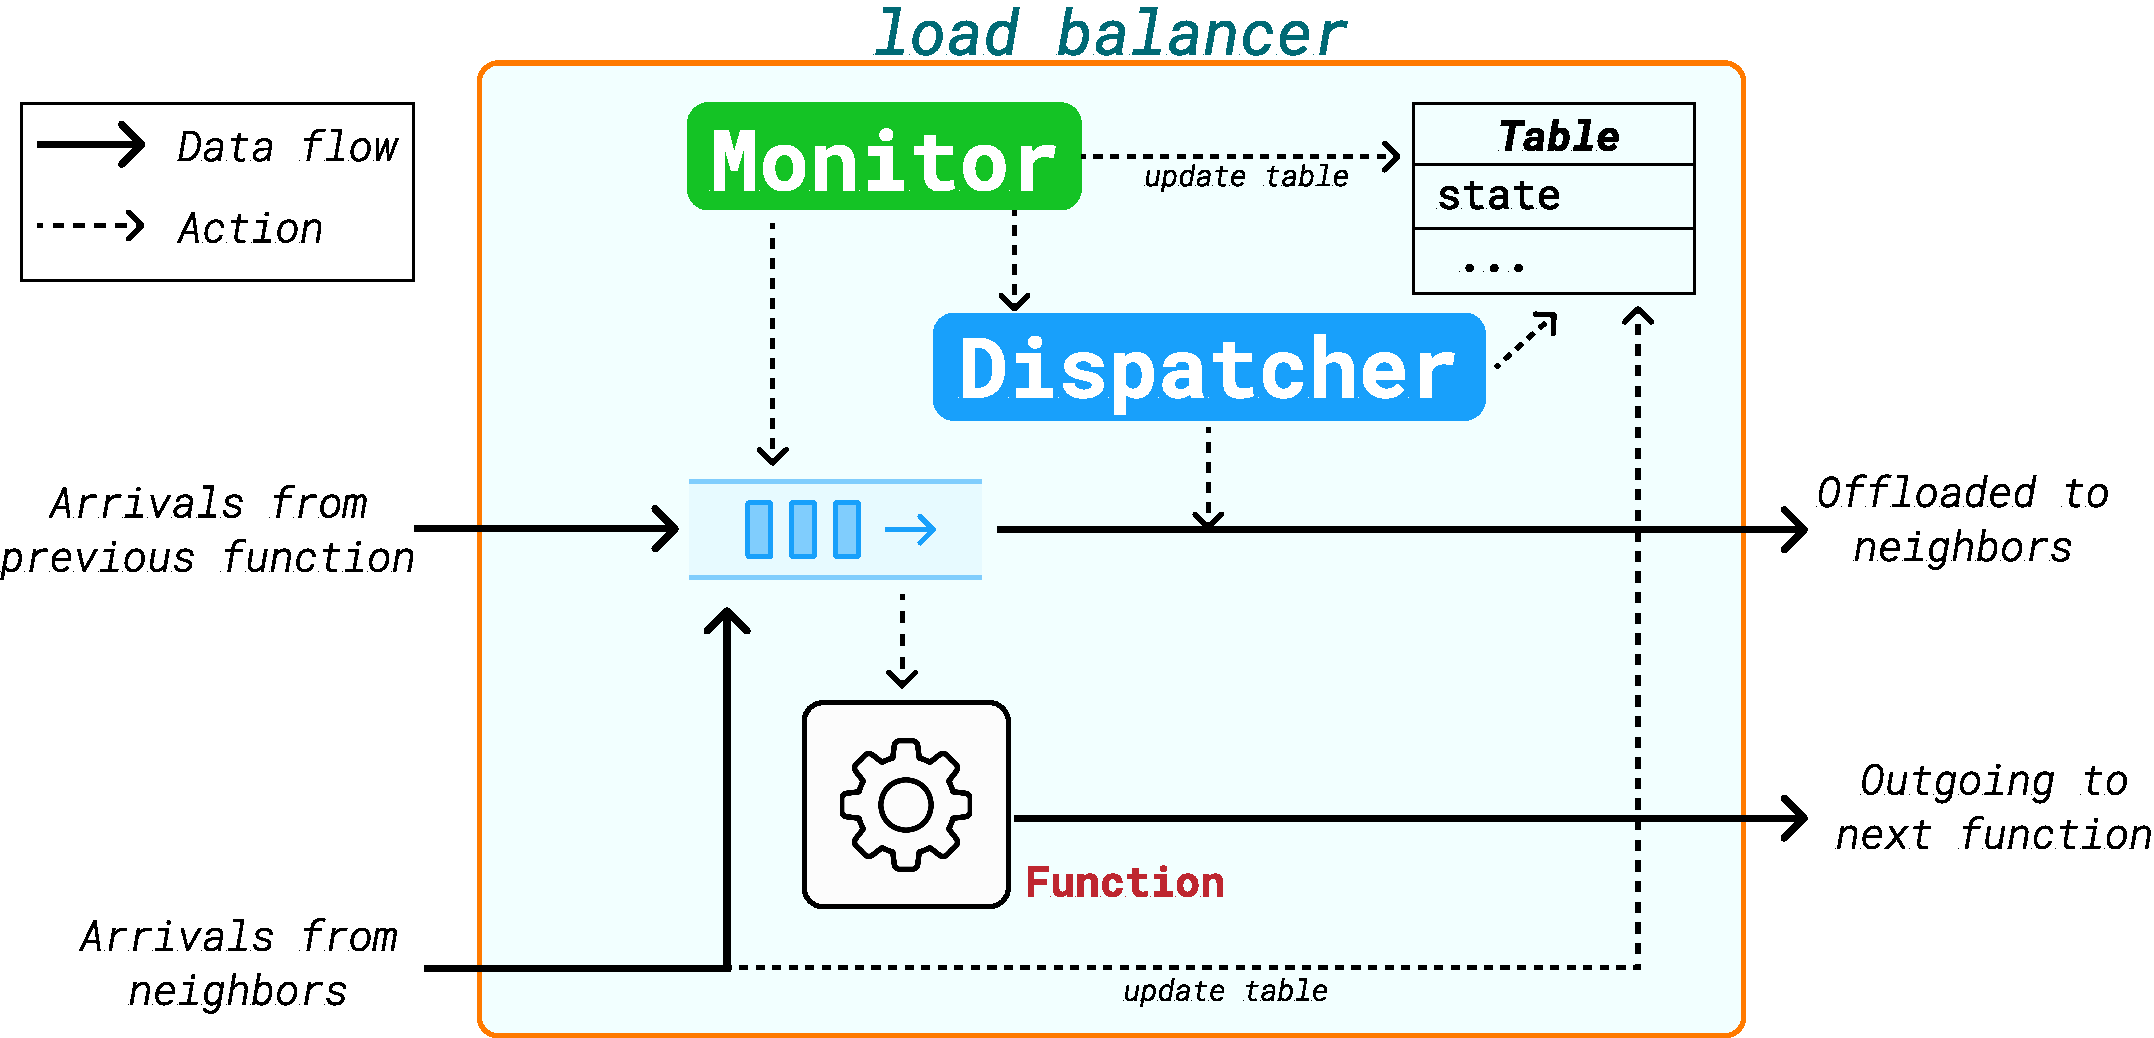
\includegraphics[width=\linewidth]{chapters/videojam/images/videojam_architecture.pdf}
    \caption{~\videojam{}'s load balancer.}
    \label{fig:load_balancer}
\end{figure}

The core~\videojam{}'s architecture leans on a set of load balancers, one associated with each and every replica the processing functions deployed among the set of available edge servers, as shown in~\Cref{fig:architecture}. In~\videojam{}, each load balancer (shown in~\Cref{fig:load_balancer}) communicates with the rest of load balancers installed on the functions of the same type (\eg, background subtractor, object recognition,~\etc), also called \textit{neighbors}. The load balancer wraps a function replica and mainly consists of two components: the \textit{Monitor} and the \textit{Dispatcher}. Through these two modules the load balancer takes decisions about incoming frames from the previous functions in the pipeline and from the neighbors to compute the (i) the output to the next function in the pipeline, and (ii) a load balancing policy, \ie, the amount of frames to be offloaded towards its neighbor. Such policy is calculated on the basis of a state table containing the information on the states of each neighbor, presented in rows. This information includes the estimates of load for the neighbors derived from predictions generated by a forecasting model. 

\subsection{Message Exchange}
In~\videojam{}'s system of load balancers, each component computes its state and load balancing policy based on local information, \ie, the incoming load from the previous function in the pipeline, and information collected from the neighbors acquired through a set of message interactions listed below. These mechanisms are designed to ensure that the load balancers converge to a common policy and compensate for potential errors in load forecasting.

\paragraph{Information Request.} Load balancers submit a request for neighbor state information when their local data is missing or obsolete. In this case, a load balancer sends, together with its table, an information request to its neighbor, asking for information about its status. Based on the response (described below), the receiver then updates its table according to the table received, substituting the rows containing obsolete information. 

\paragraph{State Update.} A state update is always sent by a load balancer in one of two scenarios: (i) at bootstrap to announce its presence to neighbors; (ii) after receiving an information request from one of its neighbors. State responses contain a summarization of the local system state, including current and forecasted loads, as well as expected incoming loads from neighbors. State updates are also sent when a prediction error is detected after receiving an offloaded workload from one of the neighbors. Such an error quantifies the difference between the expected load (according to the predictions) and the actual load received from the neighbor. 

\paragraph{Congestion Risk Signal.} A congestion risk signal is sent by a load balancer to one of its neighbors only when it detects, after updating its table and according to the last computed policy, that a given neighbor is transmitting offloaded traffic to itself, while this was not expected given previous exchanges, \ie, when the neighbor is not present in the list of neighbors from which it should receive offloaded video data.

\paragraph{Data Offloading.} Beyond the actual offloaded workload, the data transferred from a load balancer to one of its neighbors may also contain the sender's table. It is worth noting that a load balancer cannot receive workloads from the neighborhood while it is offloading to another neighbor. Hence, the receiver first checks whether it is offloading to one or more neighbors according to its computed policy. In this case, it recomputes the load balancing policy and checks whether, according to the new policy, it is supposed to receive some data. If not, it sends a congestion risk signal back to the sender. Otherwise, it receives the workload, computes the prediction error and sends a status update if the error is above a certain threshold. 

\subsection{System state computation}\label{sec:monitor}

In~\videojam{}, the system state is computed periodically and represents the current state of the load balancer based on the incoming load from the previous function in the pipeline, the processing rate, the queue size, and the offload rate to its neighbors. Here we formally describe the computation of the system state.

\paragraph{Operational Time Windows.} Each load balancer associated to function $c$, operates over a time windows $W^k_j$, which consists of $k \in \mathbb{N}^+$ consecutive time-slots and is defined as

\begin{equation*}
    W_{j} = W^k_{j} = \{w_i\}^k_{i=1},
\end{equation*}

where $w_i$ is the $i^{th}$ time-slot of the time window. All the time-slots within the time window have the same duration of $\Delta$ seconds. The next time window is denoted as $W_{j+1}$.

Each load balancer $S_{c,n}$ is characterized by its state, and keeps track of the states of all its neighbors (identified by $\mathcal{S}^*_{c}$) in a table. We further indicate with $S_{c}$ the set of all load balancers associated to function $c$ deployed among the edge nodes. 

\paragraph{State.} At each time window $W^k_{j} = \{w_i\}^k_{i=1}$, the state of load balancer $S_{c,n}$ is defined by (i) its processing rate $\mu_{c,n}$, (ii) the historical incoming load $\{\lambda^{c,n}_{w_i}\}_{w_i \in W^h_j}$ of $h \ge k$ previous time-slots, (iii) its current queue size $\varphi^{c,n}_{W_j}$, and (iv) the offload $\delta^c_n$, \ie, the total workload offloaded towards its neighbors. The table of each load balancer contains an estimation of all its neighbors' states. Such an estimation is based on the last information the load balancer has received from the neighborhood and it is updated every $r$ time windows. When this time expired, \ie, $r=0$, the load balancer sends an information request to the neighborhood. As shown in~\Cref{fig:load_balancer}, the interaction of the two main components, \ie, the Monitor and the Dispatcher, of each load balancer, determines the final offloading policy. We describe in detail how the dispatcher calculates the offloading policy in the next section.

The Monitor is in charge of monitoring the state and performance of the load balancer over time. More precisely, it supervises the incoming load from the prior function in the pipeline, and the processing rate. At each time-slot $w_i$ of a given time window, the monitor measures the amount of workload $\lambda^{c,n}_{w_i}$ coming from the previous function in the pipeline. At the end of each time window, the monitor updates the historical incoming load of the state of the load balancer by shifting its $h-k$ values to the left and replacing the last $k$ values with the load received in the window $W_{j}$. After such an update, the monitor triggers the Dispatcher for the computation of the load balancing policy.

\subsection{Load Balancer Algorithm}\label{subsec:dispatcher}
Here we describe in details the algorithm executed by each load balancer to compute its local offloading policy. The Dispatcher is in charge of computing the load balancing policy of~\videojam{} through the computation of the queue size and the prediction of future incoming workload for the load balancer. For a given function $c$, the policy is determined in such a way that the load is fairly distributed among all the load balancers in $\mathcal{S}_c$. In this manner, the load is processed at approximately the same time, as shown in~\cite{shah2007design}. Regarding the prediction of future incoming workload, given the limited capabilities of computational resources at the edge, state-of-the-art methods, such as Long Short-Term Memory (LSTM)~\cite{greff2016lstm}, result to be computationally intensive and, hence, prohibitive for the described scenario~\cite{lalapura2021recurrent}. Furthermore, when it comes to video analytics, learning the specific distribution of the load results to be a non-trivial task due to concept-drift problems~\cite{bhardwaj2022ekya},
%there is no specific distribution of load that can be learned,
especially when dealing with mobile cameras. For these reasons, the dispatcher relies on lightweight ML models to predict the incoming workload. In particular, we have developed a lightweight convolution-based neural network model based on a few convolution layers for predictions~\cite{KerasTCN}. This model presents fast inference time and high accuracy metrics. The complete pseudocode of the dispatcher is described in~\Cref{algo:dispatcher}.


\paragraph{Determine the Queue Size.} Within a given time window $W_{j}$, each load balancer determines the queue size $\varphi^{c,n}_{W_{j+1}}$, which is the load at the beginning of the next window $W_{j+1}$, by counting the amount of load currently waiting for processing (line 2 of~\Cref{algo:dispatcher}). The queue size of each neighbor $S_{c,m} \in \mathcal{S}_c^*$ is estimated
%For all $m$ in $\mathcal{S}^*_c$, the queue size is estimated 
by adding (i) the difference between the incoming load and the processing rate, and (ii) the total amount of workload exchanged with the neighborhood, to the previous expected load (lines 3--7 of~\Cref{algo:dispatcher}). More formally,
\begin{equation}
    \begin{split}
        \tilde{\varphi}^{c,m}_{W_{j+1}} = \tilde{\varphi}^{c,m}_{W_{j}} + \sum_{w_i \in W_{j}}(\lambda^{c,m}_{w_i} - \mu_{c,m}) + \delta^c_{m}, %\quad
        %\forall m \neq n, m \in \mathcal{N}, 
        %\forall w_i \in W_{k,j}}
    \end{split}
    \label{eqn:queue_size_estimation}
\end{equation}
where, $\delta^c_{m} = \sum_{p \in \mathcal{N}} \delta^c_{m \mid p}$, $\delta^c_{m \mid p}$ is the offload between $S_{c,m}$ and $S_{c,p}$, where $\delta^c_{m \mid p} < 0$ if data is offloaded from $S_{c,m}$ to $S_{c,p}$, and $\delta^c_{m \mid p} > 0$ if $S_{c,p}$ is sending data to $S_{c,m}$.

\paragraph{Predict Future Incoming Workload.} The load balancer forecasts its load and the incoming load of its neighbors for the next time window. For such predictions we rely on a convolution-based neural network model used to predict short-term workload~\cite{kombi2017preventive} (more details on the model are available in~\Cref{sec:implementation}). The input of the predictive model is the historical incoming load $W_h$ (\ie, $\{\lambda^{c,n}_{w_i}\}$ consisting of $h \ge k$ previous time-slots) for all load balancers. While the output is the incoming load for the next window $W_{j+1}$. So when the predicted workload deviates from the actual workload during the monitoring phase, the Monitor can detect it and react to make adjustments at any time.

\paragraph{Offloading Policy Computation.} 
Within a given time window $W_{j}$, each load balancer $S_{c,n}$ determines the offloading policy, \ie, $\delta_{n|m}^c$ for each $S_{c,m} \in \mathcal{S}_{c}$ for the next time-window $W_{j+1}$. Such a policy is computed through the following steps: 

(i)~First, the estimation of the global load, $\tilde{\phi}^{c,n}$, is computed according to 
\begin{equation}
    \tilde{\phi}_{c,n} = \tilde{\varphi}^{c,n}_{W_{j+1}} + \sum_{w_i \in W_{j+1}} \lambda^{c,n}_{w_i},
    \label{eqn:global_load_estimation}
\end{equation}
\ie, the estimated queue size at the beginning of the next time window plus the expected incoming load.  The queue size estimate is performed for all its neighbors in $\mathcal{S}_{c}^*$, whereas it can simply be obtained from the load balancer queue.

(ii)~Then, based on the estimation of the global load, each load balancer $S_{c,n}$ estimates the actual load that every load balancer in $\mathcal{S}_{c}$ should handle:
\begin{equation}
    \bar{\phi}_{c,n} = \frac{\sum_{n \in \mathcal{N}}\tilde{\phi}_{c,n} * \mu_{c,n}}{\sum_{n \in \mathcal{N}} \mu_{c,n}}, %\forall n \in \mathcal{N}
    \label{eqn:balanced_load_estimation}
\end{equation}
where $\tilde{\phi}_{c,n}$ is the global load that should be processed by $S_{c,n}$ with a process rate of $\mu_{c,n}$, and $\sum_{n \in \mathcal{N}} \mu_{c,n}$ is the total processing capacity of all the load balancers associated to function $c$.

(iii)~The load balancer computes the \textit{unbalanced} load for all the load balancers associated to function $c$ (line 12 in~\Cref{algo:dispatcher}) as 
\begin{equation}
    \theta_{c,n} = \bar{\phi}_{c} - \tilde{\phi}_{c,n}. %\forall n \in \mathcal{N}
    \label{eqn:unbalanced_load_estimation}
\end{equation}
Positive values for $\theta_{c,n}$ indicate that the function associated to the load balancer will be underutilized. In this case, it should receive workload from neighbors $S_{c,m}$ with negative values of $\theta_{c,m}$. Negative values for $\theta_{c,n}$, on the other hand, point out that the function will be overloaded requiring to offload some workload to the neighbors.

(iv)~Finally, the amount of workload to be offloaded towards each neighbor $S_{c,m}$, \ie, the offloading policy $\delta^c_{n \mid m}$, is finally computed based on $\theta_{c,n}$ as described from line 14 to 27 of~\Cref{algo:dispatcher}. Until all the $\theta$'s are set to $0$, the dispatcher takes the most loaded $S_{c,n}$ to balance to the least leaded $S_{c,m}$ in $S_c$. The load is transferred from $S_{c,n}$ to $S_{c,m}$ if there is enough room for the load, and the unbalanced load of $S_{c,n}$ is set to $0$. Otherwise, $S_{c,n}$ transfers to $S_{c,m}$ the maximum load that can be received $\theta_{c,m}$ and the unbalanced load of the receiver is set to $0$.

\begin{algorithm}[t]
\caption{Dispatcher algorithm procedure}
\label{algo:dispatcher}
\SetAlgoLined
\SetKwProg{Fn}{Function}{}{end} % Function name(args) [...] end
\Fn{dispatcher($\varphi$, $\lambda$, $\mu$, $\delta$, $\mathcal{S}_{c}$)}
{
\begin{small}
\tcc{1. Determine the queue size}
$\varphi^{c,n}_{W_{j+1}} = getQsize()$

\tcc{1. Estimation load for neighbors, \ie, $\mathcal{S}_c^*$}
\For{ $S_{c,m} \in \mathcal{S}_{c}^*$ } 
{
    $\tilde{\varphi}^{c,m}_{W_{j+1}} = \tilde{\varphi}^{c,m}_{W_{j}} + \sum_{w_i \in W_{j}}(\lambda^{c,m}_{w_i} - \mu_{c,m}) + \delta^c_{m}$\;
}
\For{ $S_{c,n} \in \mathcal{S}_{c}$ }
{
    \tcc{2. Forecast the future incoming load, \ie, $\lambda^{c,n}_{w_i}, w_i \in W_{j+1}$}
    $\lambda^{c,n}_{w_i} = model(\{\lambda^{c,n}_{w_i}\}_{w_i \in W^h})$\;

    \tcc{Estimation of global load}
    $\tilde{\phi}_{c,n} = \tilde{\varphi}^{c,n}_{W_{j+1}} + \sum_{w_i \in W_{j+1}} \lambda^{c,n}_{w_i}$\;
}


\tcc{Compute the unbalanced load}
\For{ $S_{c,n} \in \mathcal{S}_{c}$ }
{
    \tcc{balanced load $\bar{\phi}_{c,n}$}
    $\bar{\phi}_{c,n} = \frac{\sum_{n \in \mathcal{N}}\tilde{\phi}_{c,n} * \mu_{c,n}}{\sum_{n \in \mathcal{N}} \mu_{c,n}}$\;
    \tcc{unbalanced load}
    $\theta_{c,n} = \bar{\phi}_{c} - \tilde{\phi}_{c,n}$
}

\tcc{3. Compute the offloading policy}
\While{ $\text{any($\theta_{c,n} < 0$) and any($\theta_{c,n} > 0$)}$ }
{
    \tcc{the most overloaded}
    $n = argmin(\theta_{c})$\;
    \tcc{the less overloaded}
    $m = argmax(\theta_{c})$\;
    $q = \lvert \theta_{c,n} \lvert$\;
    \uIf{ $q < \theta_{c,m}$ }{
        \tcc{load from $S_{c,n}$ to $S_{c,m}$}
        $\delta^c_{n \mid m} = q$\;
        $\theta_{c,n} = 0$\;
        $\theta_{c,m} = \theta_{c,m} - q$\;
    }
    \Else{
        $\delta^c_{n \mid m} = \theta_{c,m}$\;
        $\theta_{c,n} = \theta_{c,n} + \theta_{c,m}$\;
        $\theta_{c,m} = 0$\;
    }
}
\end{small}
    }
\end{algorithm}
